\begin{aosachapter}{Parsing XML at the Speed of Light}{s:pugixml}{Arseny Kapoulkine}

\aosasecti{Preface}

XML is a standardized markup language that defines a set of rules for
encoding hierarchically structured documents in a human-readable
text-based format. XML is in widespread use, with documents ranging from
very short and simple (such as SOAP queries) to multi-gigabyte documents
(OpenStreetMap) with complicated data relationships (COLLADA). In order
to process XML documents, users typically need a special library: an XML
parser, which converts the document from text to internal
representation. XML is a compromise between parsing performance, human
readability and parsing-code complexity---therefore a fast XML parser
can make the choice of XML as an underlying format for application data
model more preferable.

This chapter describes various performance tricks that allowed the
author to write a very high-performing parser in C++:
\href{http://pugixml.org}{pugixml.} While the techniques were used for
an XML parser, most of them can be applied to parsers of other formats
or even unrelated software (e.g., memory management algorithms are
widely applicable beyond parsers).

Since there are several substantially different approaches to XML
parsing, and the parser has to do additional processing that even people
familiar with XML do not know about, it is important to outline the
entire task at hand first, before diving into implementation details.

\aosasecti{XML parsing models}

Each of the different models of XML parsing is appropriate in different
situations, and each has implications for performance and memory
consumption. The following models are in widespread use:

\begin{aosaitemize}

\item
  With SAX (Simple API for XML) parsers, the user provides the parser
  with a document stream as an input and several callbacks such as
  ``start of tag,'' ``end of tag,'' ``character data inside tag''. The
  parser invokes the callbacks according to the data in the document.
  The context needed for parsing is limited by the tree depth of the
  current element, which means that the memory requirements are greatly
  reduced. This type of parsing can be used for streaming documents
  where only part of the document is available at any single time.
\item
  Pull parsing is similar to SAX in the parsing process---that is, the
  document is processed one element at a time---but the control is
  inverted: in SAX, parsing is controlled by the parser through
  callbacks, whereas in Pull parsing the user controls the parsing
  process through an iterator-like object.
\item
  With DOM (Document Object Model) parsers, the user provides the parser
  with the entire document as a text stream/buffer, from which the
  parser generates a document object---an in-memory representation of
  the entire document tree, which has an individual object for each
  specific XML element or attribute, and a set of allowed operations
  (e.g., ``get all child elements of this node''). Pugixml follows this
  model.
\end{aosaitemize}

The choice of the parsing model usually depends on the document size and
structure. Since pugixml is a DOM parser, it is effective for documents
that:

\begin{aosaitemize}

\item
  are small enough to fit in memory,
\item
  have a complicated structure with references between nodes that need
  to be traversed, or
\item
  need complicated document transformations.
\end{aosaitemize}

\aosasecti{Design choices in pugixml}

Pugixml focuses on the problem of DOM parsing largely because, while
fast and lightweight SAX parsers (such as Expat) were available, all
production-ready XML DOM parsers at the time of pugixml's creation
(2006) were either not very lightweight, not very fast
or---usually---neither. Thus the main goal of pugixml is to be a very
fast lightweight DOM-based XML manipulation library.

XML is defined by a \href{http://www.w3.org/TR/REC-xml/}{W3C
recommendation} that specifies two different types of parsing:
validating and non-validating (in other words, non-validating parsers
check XML syntax while validating parsers can check data semantics as
well). Even a non-validating parser has to do some relatively
resource-intensive validation work.

When performance is the primary goal, a compromise must be reached
between performance and conformance. For pugixml the compromise is as
follows: any well-formed XML document will be fully parsed, including
all required transformations, with the exception of document type
declarations.\footnote{Document type (DOCTYPE) declarations are parsed
  but their contents are ignored. This decision is based on performance
  issues, implementation complexity and demand for the feature.} Since
only rules that are fast to verify are checked, a non-well-formed
document can sometimes be parsed successfully.

The data in an XML document often has to be transformed in certain ways
by the time it reaches the user. The transformations include end-of-line
handling, attribute-value normalization and character reference
expansion. These transformations have an associated performance cost;
pugixml optimizes them as much as possible while providing a way to
disable them for maximum performance.

The task at hand is to make a fast DOM parser that successfully parses
conforming XML documents with required transformations, is as fast as
reasonably possible, and is production ready. For performance purposes,
``production ready'' mainly means it offers resistance to malformed
data. Sacrificing buffer overrun checks to improve performance is not
feasible.

Next, we'll discuss the parsing process used by pugixml. The last
sections will describe the data structure used by pugixml to store the
document object model and the algorithm used by pugixml to allocate
memory for this data structure.

\aosasecti{Parsing}

The goal of a DOM parser is to take an input---a string that contains an
XML document---and produce a tree of objects that represents the same
document in memory. A parser typically consists of two stages: a lexer
and a parser. A lexer is given an input character stream and produces a
token stream. (For an XML parser the set of tokens can include open
angle brackets, quotation marks, tag names, and attribute names.) The
parser consumes the token stream and produces a syntax tree based on the
grammar, using one of many parsing algorithms such as recursive descent.
When encountering a token with string data, such as a tag name, the
lexer or parser copies the string contents to a heap and stores a
reference to the string inside a tree node.

To improve parsing performance, pugixml deviates from the typical
approach in several ways.

\aosasectii{Token stream vs.~character stream}

As mentioned before, parsers traditionally use lexers to convert the
character stream into a token stream. This can improve performance in
cases where a parser has to do a lot of backtracking, but for XML
parsers a lexer stage is just an extra layer of complexity that
increases the per-character overhead. Thus pugixml operates on a
character stream instead of a token stream.

Normally a stream consists of UTF-8 characters, and pugixml reads the
stream byte by byte. Due to UTF-8 structure there is no need to parse
UTF-8 byte sequences unless you're looking for specific non-ASCII
characters, because in valid UTF-8 streams all bytes below 128 are
standalone ASCII characters (i.e., are not part of a UTF-8
character).\footnote{Note that conforming XML parsers are required to
  reject certain Unicode codepoints. Pugixml sacrifices this analysis
  for increased performance.}

\aosasectii{In-place parsing}

There are several inefficiencies in the typical implementation of a
parser. One of them is copying string data to the heap. This involves
allocating many blocks of varying sizes, from bytes to megabytes, and
requires us to copy all strings from the original stream to the heap.
Avoiding the copy operation allows us to eliminate both sources of
overhead. Using a technique known as in-place (or \emph{in situ})
parsing, the parser can use data from the stream directly. This is the
parsing strategy used by pugixml.

A basic in-place parser takes an input string stored in a contiguous
memory buffer, scans the string as a character stream, and creates the
necessary tree structure. Upon encountering a string that is part of the
data model, such as a tag name, the parser saves a pointer to the string
and its length (instead of saving the whole string).\footnote{This
  creates a lifetime dependency---the entire source buffer must outlive
  all document nodes for the technique to work.}

As such, this is a tradeoff between performance and memory usage.
In-place parsing is usually faster compared to parsing with copying
strings to the heap, but it can consume more memory. An in-place parser
needs to hold the original stream in memory in addition to its own data
describing the document's structure. A non in-place parser can store
relevant parts of the original stream instead.

\begin{figure}[htbp]
\centering
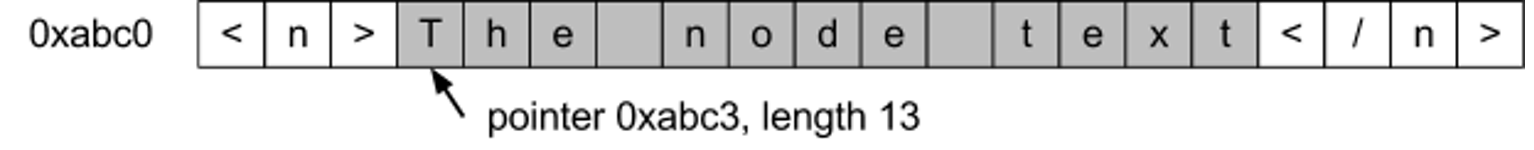
\includegraphics{pugixml-images/image01.png}
\caption{An example of basic in-place text parsing.}
\end{figure}

Most in-place parsers have to deal with additional issues. In the case
of pugixml, there are two: simplifying string access and transforming
XML data during parsing.

Accessing strings that are parsed in-place is difficult because they are
not null-terminated. That is, the character after the string is not a
null byte, but is instead the next character in the XML document, such
as an open angle bracket (\texttt{\textless{}}). This makes it difficult
to use standard C/C++ string functions that expect null-terminated
strings.

To make sure we can use these functions we'll have to null-terminate the
strings during parsing. Since we can't easily insert new characters, the
character after the last character of each string will have to be
overwritten with a null character. Fortunately, we can always do this in
XML: a character that follows the end of a string is always a markup
character and is never relevant to document representation in memory.

\begin{figure}[htbp]
\centering
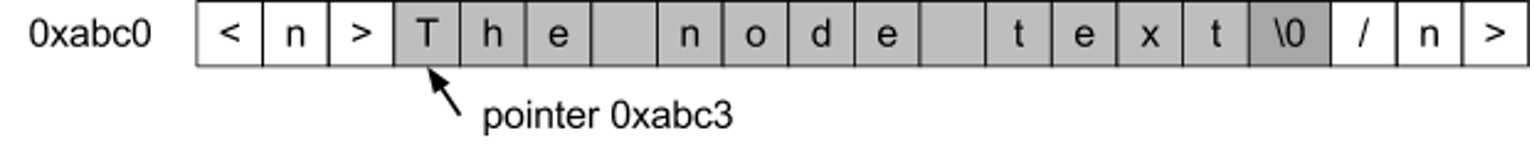
\includegraphics{pugixml-images/image03.png}
\caption{Adjusting in-place parsing for null-terminated strings.}
\end{figure}

The second issue is more complicated: often the string value and the
representation in the XML file are different. A conforming parser is
expected to perform decoding of the representation. Since doing this
during node object access would make object access performance
unpredictable, we prefer to do this at parsing time. Depending on the
content type, an XML parser could be required to perform the following
transformations:

\begin{aosaitemize}
\item
  End-of-line handling: The input document can contain various types of
  line endings and the parser should normalize them as follows: any
  two-character sequence of one carriage return (ASCII 0xD) and one line
  feed (ASCII 0xA) and any free-standing carriage return should be
  replaced with a line feed character. For example, the line

\begin{verbatim}
  `line1\xD\xAline2\xDline3\xA\xA`
\end{verbatim}

  should be transformed to

\begin{verbatim}
  `line1\xAline2\xAline3\xA\xA`.
\end{verbatim}
\item
  Character reference expansion: XML supports escaping characters using
  their Unicode code point with either decimal or hexadecimal
  representation. For example, \texttt{\&\#97;} should expand to
  \texttt{a} and \texttt{\&\#xf8;} should expand to ø.
\item
  Entity reference expansion: XML supports generic entity references,
  where \&name; is replaced with the value of entity name. There are
  five predefined entities: \texttt{\&lt;} (\textless{}), \texttt{\&gt;}
  (\textgreater{}), \texttt{\&quot;} (``), \texttt{\&apos;} (') and
  \texttt{\&amp;} (\&).
\item
  Attribute-value normalization: in addition to expanding references,
  the parser should perform whitespace normalization when parsing
  attribute values. All whitespace characters (space, tab, carriage
  return and line feed) should be replaced with a space. Additionally,
  depending on the type of the attribute, leading and trailing
  whitespaces should be removed and whitespace sequences in the middle
  of the string should be collapsed into a single space.
\end{aosaitemize}

It is possible to support an arbitrary transformation in an in-place
parser by modifying the string contents, given an important constraint:
a transformation must never increase the length of the string. If it
does, the result might overlap with significant data in the document.
Fortunately, all of the above transformations satisfy this
requirement.\footnote{This is obvious for all transformations, except
  perhaps Unicode transformation. In that case, both UTF-8 and UTF-16
  encodings are more compact than hexadecimal or decimal representation
  of Unicode code points, which is why replacing one with the other
  never increases the length.}

General entity expansion does \emph{not} satisfy this constraint. Since
pugixml does not support \texttt{DOCTYPE} declarations, and it is
impossible to specify custom entities without \texttt{DOCTYPE}, any
supported document can be fully parsed using in-place parsing.\footnote{It
  is possible to support general entity references with in-place parsing
  by splitting every string with an entity reference into three nodes:
  prefix string before entity reference, a node of a special type that
  contains the reference id, and a suffix string, which may have to be
  split further. This approach is used by the Microsoft XML parser (for
  different reasons).}

\begin{figure}[htbp]
\centering
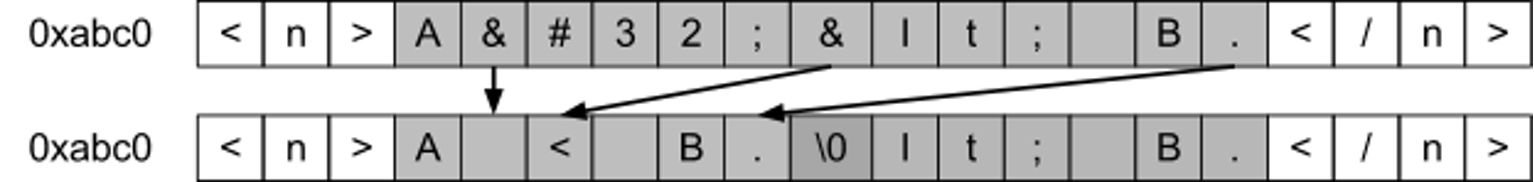
\includegraphics{pugixml-images/image04.png}
\caption{Text transformations with in-place text parsing.}
\end{figure}

Interestingly, in-place parsing can be used with memory-mapped file
I/O.\footnote{See \url{http://en.wikipedia.org/wiki/Memory-mapped_file}.}
Supporting null-termination and text transformation requires a special
memory mapping mode known as \emph{copy-on-write} to avoid modifying the
file on disk.

Using memory mapped file I/O with in-place parsing has the following
benefits:

\begin{aosaitemize}

\item
  The kernel can usually map cache pages directly into the process
  address space, thus eliminating a memory copy that would have happened
  with standard file I/O.
\item
  If the file is not already in the cache, the kernel can prefetch
  sections of the file from disk, effectively making I/O and parsing
  parallel.
\item
  Since only modified pages need to allocate physical memory, memory
  consumption can be greatly decreased on documents with large text
  sections.
\end{aosaitemize}

\aosasectii{Optimizing character-wise operations}

Eliminating string copies is not the only thing we can do to optimize
parser performance. When comparing parser performance, a useful metric
is the average number of processor cycles spent for each character.
While this varies among documents and processor architectures, it is
reasonably stable for documents of similar structure. Thus it makes
sense to optimize for this metric, and an obvious place to start is in
the operations performed for each character.

The most important operation is detecting character set membership:
given a character from the input stream, does it belong to a certain set
of characters?

A useful approach is to create a Boolean flag table, where for each
character value a true/false value is stored depending on whether the
character belongs to the set or not. Depending on the encoding,
different table data structures and sizes make sense as follows:

\begin{aosaitemize}
\item
  For encodings where each character occupies no more than 8 bits, a
  table of size 256 is sufficient.
\item
  For UTF-8, we would like to use a byte-indexed table to avoid code
  point decoding; this works only if all characters with code points
  (i.e.~numeric values) above 127 belong to the set or no characters
  with code points above 127 belong to the set. If either of these are
  true, then a table of size 256 is sufficient. The first 128 entries of
  the table are filled with true or false (depending on whether the
  character is in the target set) and the last 128 entries of the table
  all share the same value. Because of the way UTF-8 encodes data, all
  code points above 127 will be represented as sequences of bytes with
  values above 127. Furthermore, the first character of the sequence
  will also be above 127.
\item
  For UTF-16 or UTF-32, tables of large sizes are usually impractical.
  Given the same constraint as the one for optimized UTF-8, we can leave
  the table to be 128 or 256 entries large, and add an additional
  comparison to deal with values outside the range.
\end{aosaitemize}

Note that we only need one bit to store the true/false value, so it
might make sense to use bitmasks to store eight different character sets
in one 256 byte table. Pugixml uses this approach to save cache space:
on the x86 architecture, checking a boolean value usually has the same
cost as checking a bit within a byte, provided that bit position is a
compile-time constant. This C code demonstrates this approach:

\begin{verbatim}
enum chartype_t {
  ct_parse_pcdata  = 1, // \0, &, \\r, \<
  ct_parse_attr    = 2, // \0, &, \\r, ', "
  ct_parse_attr_ws = 4, // \0, &, \\r, ', ", \\n, tab
  // ...
};
static const unsigned char table[256] = {
  55, 0, 0, 0, 0, 0, 0, 0, 0, 12, 12, 0, 0, 63, 0, 0, // 0-15
  // ...
};
bool ischartype_utf8(char c, chartype_t ct) {
  // note: unsigned cast is important to
  // guarantee that the value is in 0..255 range
  return ct & table[(unsigned char)c];
}

bool ischartype_utf16_32(wchar_t c, chartype_t ct) {
  // note: unsigned cast is important to
  // guarantee that the value is not negative
  return ct & ((unsigned)c < 128 ? table[(unsigned)c] : table[128]);
}
\end{verbatim}

If the tested range includes all characters in a certain interval, it
might make sense to use a comparison instead of a table lookup. With
careful use of unsigned arithmetics just one comparison is needed. For
example, a test for a character being a digit:

\begin{verbatim}
bool isdigit(char ch) { return (ch >= '0' && ch <= '9'); }
\end{verbatim}

\noindent can be rewritten using just one comparison:

\begin{verbatim}
bool isdigit(char ch) { return (unsigned)(ch - '0') < 10; }
\end{verbatim}

If we work character by character, improving on the above approaches is
usually impossible. However, it is sometimes possible to work on groups
of characters and use vectorized checks. If the target system has some
form of SIMD instructions available, you can usually use these
instructions for fast operation on groups of 16 characters or more.

Even without resorting to platform-specific instruction sets it is
sometimes possible to vectorize character operations. For example, here
is one way to check if four consecutive bytes in a UTF-8 byte stream
represent ASCII symbols\footnote{Of course, the data has to be suitably
  aligned for this to work; additionally, this technique violates strict
  aliasing rules of the C/C++ standard, which may or may not be a
  problem in practice.

  (\emph{(const uint32\_t})data \& 0x80808080) == 0}:

Finally, whatever you do, avoid \texttt{is.*()} functions from the
standard library (such as \texttt{isalpha()}) for performance-sensitive
code. Even the best implementations check whether the current locale is
``C'', which is more expensive than the table lookup itself, and the
worst implementations can be two orders of magnitude slower than
that.\footnote{See \aosachapref{s:khmer} for another example of this
  problem.}

\aosasectii{Optimizing string transformations}

In pugixml, the reading and transformation of values is particularly
time-consuming. For example, let's look at reading plain-character data
(PCDATA); e.g., the text between the XML tags. Any standard conforming
parser, as previously discussed, should perform reference expansion and
end of line normalization during PCDATA content processing.\footnote{Pugixml
  allows the user to turn either of these off at runtime for both
  performance and data preservation reasons. For example, you might be
  dealing with documents where it is important to preserve the exact
  type of newline sequences, or where entity references should be left
  unexpanded by the XML parser in order to be processed afterwards.}

For example, the following text in XML:

\begin{verbatim}
A&#32;&lt; B.
\end{verbatim}

\noindent should be transformed to

\begin{verbatim}
A < B.
\end{verbatim}

The PCDATA parsing function takes a pointer to the start of PCDATA
value, and proceeds by reading the rest of the value, converting the
value data in-place and null-terminating the result.

Since there are two boolean flags, we have four variations of this
function. In order to avoid expensive run-time checks, we're using
boolean template arguments for these flags---thus we're compiling four
variations of a function from a single template, and then using runtime
dispatch to obtain the correct function pointer once before the parsing
begins. The parser calls the function using this function pointer.

This allows the compiler to remove condition checks for flags and remove
dead code for each specialization of the function. Importantly, inside
the function's parsing loop we use a fast character set test to skip all
characters that are part of the usual PCDATA content, and only process
the characters we're interested in. Here's what the code looks like:

\begin{verbatim}
template <bool opt_eol, bool opt_escape> struct
strconv_pcdata_impl {
  static char_t* parse(char_t* s) {
    gap g;
    while (true) {
      while (!PUGI__IS_CHARTYPE(*s, ct_parse_pcdata)) ++s;
      if (*s == '<') { // PCDATA ends here
        *g.flush(s) = 0;
        return s + 1;
      } else if (opt_eol && *s == '\r') { // 0x0d or 0x0d 0x0a pair
        *s++ = '\n'; // replace first one with 0x0a
        if (*s == '\n') g.push(s, 1);
      } else if (opt_escape && *s == '&') {
        s = strconv_escape(s, g);
      } else if (*s == 0) {
        return s;
      } else {
        ++s;
      }
    }
  }
};
\end{verbatim}

\noindent An additional function gets a pointer to a suitable
implementation based on runtime flags; e.g.,
\texttt{\&strconv\_pcdata\_impl\textless{}false, true\textgreater{}::parse}.

One unusual item in this code is the \texttt{gap} class instance. As
shown before, if we do string transformations, the resulting string
becomes shorter because some of the characters have to be removed. There
are several ways of doing this.

One strategy (that pugixml \emph{doesn't} use) is to keep separate
\texttt{read} and \texttt{write} pointers that both point to the same
buffer. In this case the \texttt{read} pointer tracks the current read
position, and the \texttt{write} pointer tracks the current write
position. At all times the invariant \texttt{write \textless{}= read}
should hold. Any character that has to be a part of the resulting string
must be explicitly written to the write pointer. This technique avoids
the quadratic cost of naive character removal, but is still inefficient,
since we now read and write all characters in the string every time,
even if we don't need to modify the string.

An obvious extension of this idea is to skip the prefix of the original
string that does not need to be modified and only start writing
characters after that prefix---indeed, that's how algorithms like the
one behind \texttt{std::remove\_if()} commonly operate.

Pugixml follows a different approach (see
\aosafigref{posa.pugixml.gapops}). At any time there is \emph{at most
one gap} in the string. The gap is a sequence of characters that are no
longer valid because they are no longer part of the final string. When a
new gap has to be added because another substitution was made (e.g.,
replacing \texttt{\&quot;} with " generates a gap of 5 characters), the
existing gap (if one exists) is collapsed by moving the data between two
gaps to the beginning of the first gap and then remembering the new gap.
In terms of complexity, this approach is equivalent to the approach with
read and write pointers; however it allows us to use faster routines to
collapse gaps. (Pugixml uses memmove which can copy more efficiently
compared to a character-wise loop, depending on the gap length and on C
runtime implementation.)

\aosafigure{pugixml-images/image02.png}{An example of gap operations during PCDATA conversion.}{posa.pugixml.gapops}

\aosasectii{Optimizing control flow}

The pugixml parser itself can be thought of as a recursive-descent
parser. However, the recursion is transformed into a loop to improve
performance. A node cursor acts as a stack. When a start tag is
encountered, a new node is appended to the cursor and becomes the new
cursor; when an end tag is encountered, the cursor is moved to the
parent of the current cursor. This makes stack space consumption
constant regardless of the input document, which improves robustness,
and avoids potentially expensive function calls.

The parser uses a dispatch loop that reads a character from the stream,
reads zero or more characters past that (depending on the first
character) to determine the tag type, and then proceeds to the code that
parses the relevant tag. For example, if the first character is
\texttt{\textless{}}, we have to read at least one more character to
differentiate between a start tag, end tag, comment, or other types of
tags. Pugixml also uses \texttt{goto} statements to avoid going through
the dispatch loop in certain cases --- for example, text content parsing
stops at the end of stream or the \texttt{\textless{}} character.
However, if the next character is \texttt{\textless{}}, we don't have to
go through the dispatch loop only to read the character again and check
that it's \texttt{\textless{}}; we can jump straight to the code that
does the tag parsing.

Two important optimizations for such code are branch ordering and code
locality.

In the parser, various parts of the code handle various forms of inputs.
Some of them (such as tag name or attribute parsing) execute frequently,
while others (such as DOCTYPE parsing) rarely execute at all. Even
within a small section of code, different inputs have different
probabilities. For example, after the parser encounters an open angle
bracket (\texttt{\textless{}}), the most likely character to appear next
is a character of a tag name. Next most likely is \texttt{/}\footnote{The
  reason \texttt{/} is less probable than a tag name character is that
  for every end tag there is a start tag, but there are also
  empty-element tags such as \texttt{\textless{}node/\textgreater{}}.},
followed by \texttt{!} and \texttt{?}.

With this in mind, it is possible to rearrange the code to yield faster
execution. First, all ``cold'' code; that is, code that is unlikely to
ever execute, or is unlikely to execute frequently---in the case of
pugixml this includes all XML content except element tags with
attributes and text content --- has to be moved out of the parser loop
into separate functions. Depending on the function's contents and the
compiler, adding attributes such as \texttt{noinline}, or specifically
marking extra functions as ``cold'' might help. The idea is to limit the
amount of code inlined into the main parser function to the hot code.
This helps the compiler optimize the function by keeping the control
flow graphs small, and keeps all hot code as close together as possible
to minimize instruction cache misses.

After this, in both hot and cold code it makes sense to order any
conditional chains you have by condition probability. For example, code
like this is not efficient for typical XML content:

\begin{verbatim}
if (data[0] == '<')
{
  if (data[1] == '!') { ... }
  else if (data[1] == '/') { ... }
  else if (data[1] == '?') { ... }
  else { /* start-tag or unrecognized tag */ }
}
\end{verbatim}

\noindent A better version would look like this:

\begin{verbatim}
if (data[0] == '<')
{
  if (PUGI__IS_CHARTYPE(data[1], ct_start_symbol)) { /* start-tag */ }
    else if (data[1] == '/') { ... }
    else if (data[1] == '!') { ... }
    else if (data[1] == '?') { ... }
    else { /* unrecognized tag */ }
}
\end{verbatim}

\noindent In this version the branches are sorted by probability from
most-frequent to least-frequent. This minimizes the average amount of
condition tests and conditional jumps performed.

\aosasectii{Ensuring memory safety}

Memory safety is an important concern for a parser. On any input
(including malformed input), the parser must never read or write memory
beyond the end of the input buffer. There are two ways to implement
this. The first option is to make sure the parser checks the current
read position against the end position everywhere. The second option is
to use a null-terminated string as an input and make sure the parser
handles the null terminator accordingly. Pugixml uses an extended
variant of the latter.

Additional read position checks incur a noticeable performance overhead,
whereas the null terminator is often naturally included in existing
checks. For example, the loop

\begin{verbatim}
while (PUGI__IS_CHARTYPE(*s, ct_alpha))
  ++s;
\end{verbatim}

\noindent skips a run of alphabetical characters and stops at the null
terminator or the next non-alphabetic character without requiring extra
checks. Storing the buffer end position everywhere also reduces the
overall speed because it usually requires an extra register. Function
calls also get more expensive since you need to pass two pointers
(current position and end position) instead of one.

However, requiring null-terminated input is less convenient for library
users: often XML data gets read into a buffer that might not have space
for an extra null terminator. From the client's point of view a memory
buffer should be a pointer and a size with no null terminator.

Since the internal memory buffer has to be mutable for in-place parsing
to work, pugixml solves this problem in a simple way. Before parsing, it
replaces the last character in the buffer with a null terminator and
keeps track of the value of the old character. That way, the only places
it has to account for the value of the last character are places where
it is valid for the document to end. For XML, there are not
many\footnote{For example, if a tag name scan stopped at the null
  terminator, then the document is invalid because there are no valid
  XML documents where the character before the last one is a part of tag
  name.}, so the approach results in a net win.\footnote{Of course, the
  parsing code becomes more complicated, since some comparisons need to
  account for the value of the last character, and all others need to
  skip it for performance reasons. A unit test suite with good coverage
  and fuzz testing helps keep the parser correct for all document
  inputs.}

This summarizes the most interesting tricks and design decisions that
help keep pugixml parser fast for a wide range of documents. However,
there is one last performance-sensitive component of the parser that is
worth discussing.

\aosasecti{Data structures for the document object model}

An XML document is a tree-like structure. It contains one or more nodes;
each node can contain one or more nodes; nodes can represent different
types of XML data, such as elements or text; and element nodes can also
contain one or more attributes.

Every representation of node data is usually a tradeoff between memory
consumption and the performance of various operations. For example,
\emph{semantically} a node contains a collection of child nodes; this
collection can be represented in the data structure. Specifically, this
data can be stored as an array or as a linked list. An array
representation would allow for fast index-based access; a linked list
representation would allow for constant-time insertions or
removals.\footnote{Tree modification is important---while there are ways
  to represent immutable trees much more efficiently compared to what
  pugixml is doing, tree mutation is a much needed feature both for
  constructing documents from scratch and for modifying existing
  documents.}

Pugixml chooses to represent both node and attribute collections as a
linked list. Why not as arrays? The two main benefits of arrays are fast
index-based access (which is not particularly important for pugixml) and
memory locality (which can be achieved through different means).

Fast index-based access is usually not needed because the code that
processes the XML tree either needs to iterate through all child nodes
or get a specific node that is identified by the value of an attribute
(e.g. ``get the child node with an `id' attribute equal to
`X'\,'').\footnote{More complex logic can be used as well.} Index-based
access is also fragile in a mutable XML document: for example, adding
XML comments alters the indices of subsequent nodes in the same subtree.

Memory locality depends on the allocation algorithm. With the right
algorithm, linked lists can be as efficient as arrays if list nodes are
allocated sequentially. (More on this later.)

The basic tree data structure with children stored in an array (which is
\emph{not} what pugixml uses) usually looks like this:\footnote{The
  capacity field is required to implement an amortized constant-time
  addition. See \mbox{\url{http://en.wikipedia.org/wiki/Dynamic_array}}
  for more information.

  struct Node \{ Node* children; size\_t children\_size; size\_t
  children\_capacity; \};}

The basic tree data structure that uses linked lists (which is not
\emph{exactly} what pugixml uses) looks like this:

\begin{verbatim}
struct Node {
  Node* first_child;
  Node* last_child;
  Node* prev_sibling;
  Node* next_sibling;
};
\end{verbatim}

Here, the \texttt{last\_child} pointer is necessary to support backwards
iteration and appending in O(1) time.

Note that with this design it is easy to support different node types to
reduce memory consumption; for example, an element node needs an
attribute list but a text node does not. The array approach forces us to
keep the size of all node types the same, which prevents such
optimization from being effective.

Pugixml uses a linked list-based approach. That way, node modification
is always O(1). Furthermore, the array approach would force us to
allocate blocks of varying sizes, ranging from tens of bytes to
megabytes in case of a single node with a lot of children; whereas in
the linked list approach there are only a few different allocation sizes
needed for node structure. Designing a fast allocator for fixed size
allocations is usually easier than designing a fast allocator for
arbitrary allocations which is another reason pugixml chooses this
strategy.

To keep memory consumption closer to the array-based approach, pugixml
omits the \texttt{last\_child} pointer, but keeps access to the last
child available in O(1) time by making the sibling list partially cyclic
with \texttt{prev\_sibling\_cyclic}:

\begin{verbatim}
struct Node {
  Node* first_child;
  Node* prev_sibling_cyclic;
  Node* next_sibling;
};
\end{verbatim}

\noindent This data structure is organized as follows:

\begin{aosaenumerate}
\def\labelenumi{\arabic{enumi}.}

\item
  \texttt{first\_child} points to the first child of the node, or
  \texttt{NULL} if node has no children.
\item
  \texttt{prev\_sibling\_cyclic} points to the left sibling of the node
  (a child of node's parent that is immediately before the node in the
  document). If the node is the leftmost one (i.e., if the node is the
  first child of its parent), \texttt{prev\_sibling\_cyclic} points to
  the last child of the node's parent, or to itself if it is the only
  child. \texttt{prev\_sibling\_cyclic} cannot be \texttt{NULL}.
\item
  \texttt{next\_sibling} points to the right sibling of the node or
  \texttt{NULL} if the node is the last child of its parent.
\end{aosaenumerate}

\begin{figure}[htbp]
\centering
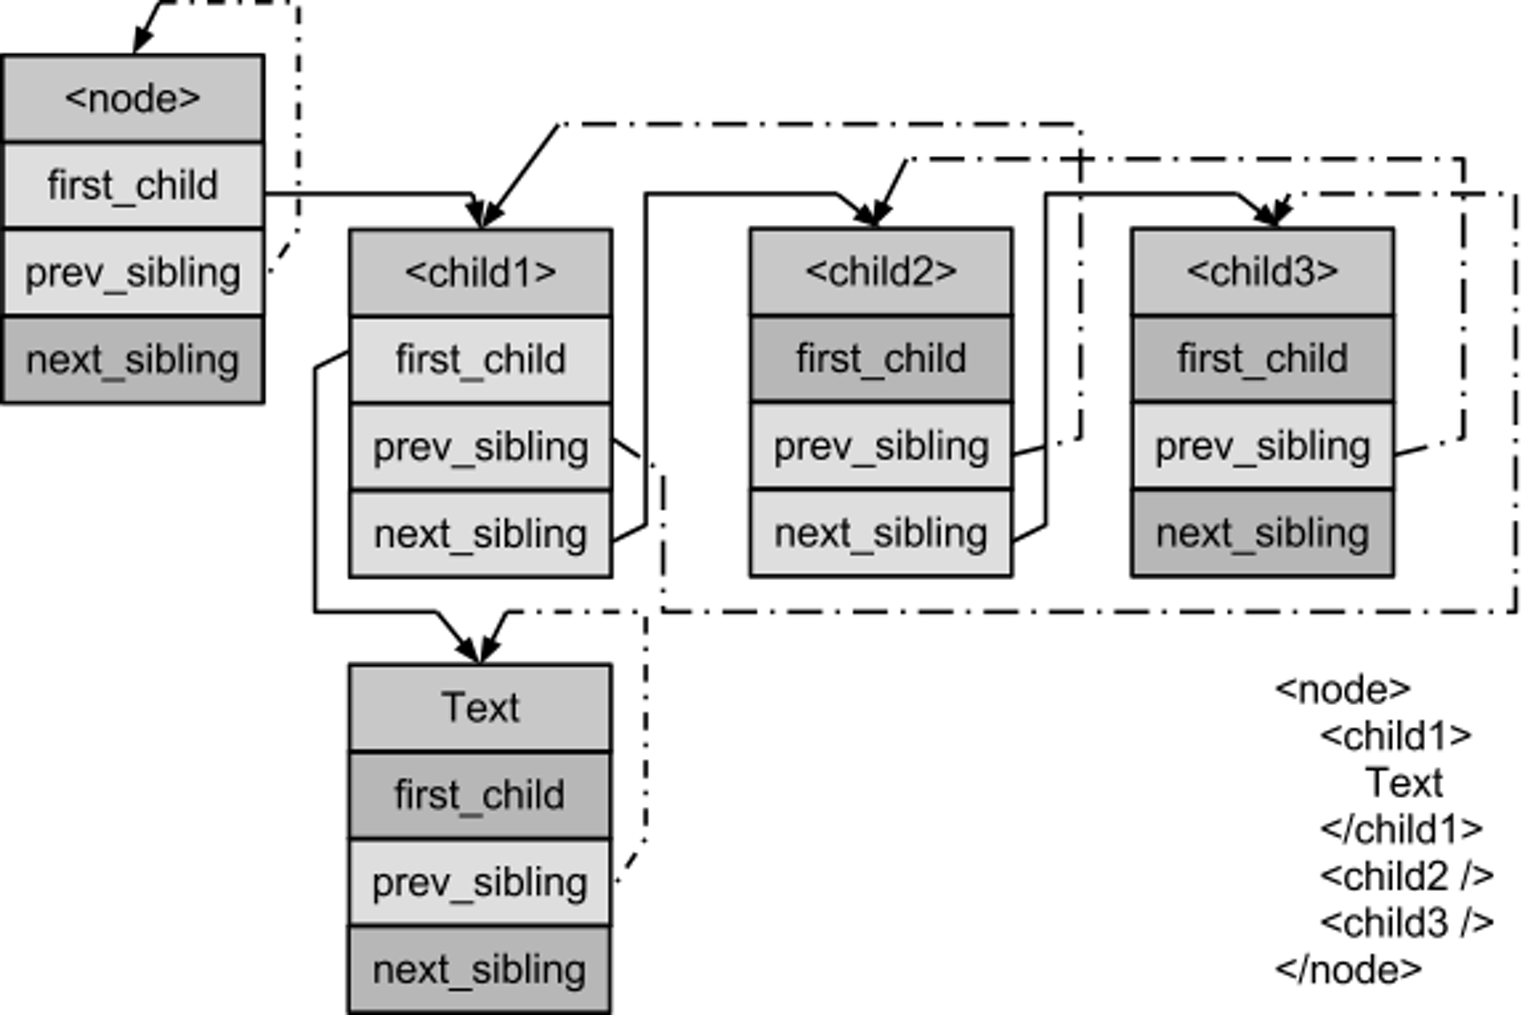
\includegraphics{pugixml-images/image00.png}
\caption{An example subtree, represented using partially-cyclic linked
lists.}
\end{figure}

\noindent With this structure, all of the following operations are
constant-time:

\begin{verbatim}
Node* last_child(Node* node) {
  return (node->first_child) ?
      node->first_child->prev_sibling_cyclic : NULL;
}

Node* prev_sibling(Node* node) {
  return (node->prev_sibling_cyclic->next_sibling) ?
      node->prev_sibling_cyclic : NULL;
}
\end{verbatim}

The array-based approach and the linked list approach with the
partially-cyclic-sibling-list trick become equivalent in terms of memory
consumption. Using 32-bit types for size/capacity makes the array-based
node smaller on 64-bit systems.\footnote{This assumes a limit of $2^{32}$
  child nodes.} In the case of pugixml, other benefits of linked lists
outweigh the costs.

With the data structures in place, it is time to talk about the last
piece of the puzzle---the memory allocation algorithm.

\aosasecti{Stack-based memory allocation}

A fast memory allocator is critical for the performance of a DOM parser.
In-place parsing eliminates allocation for string data, but DOM nodes
still need to be allocated. String allocations of varying sizes are also
needed to support tree mutation. Preserving allocation locality is
important for tree traversal performance: if successive allocation
requests return adjacent memory blocks, it becomes easy to ensure tree
locality during construction. Finally, destruction speed is important:
in addition to deletion in constant time, the ability to quickly
deallocate all memory allocated for the document without deleting each
node individually can significantly improve the time it takes to destroy
large documents.

Before discussing the allocation scheme that pugixml uses, let's discuss
a scheme that it \emph{could} have used.

Since DOM nodes have a small set of required allocation sizes, it would
be possible to use a standard memory pool based on free lists for each
size. For such a pool, there would be a single linked list of free
blocks where each block is the same size. During an allocation request,
if the free list is empty, a new page with an array of blocks is
allocated. The blocks are linked together to form a single linked list,
which then becomes the free list of the allocator. If a free list is not
empty, the first block is removed from the list and returned to the
user. A deallocation request simply prepends the block to the free list.

This allocation scheme is very good at reusing memory---allocating a
node after freeing some other node would reuse the memory immediately.
However, adding support for releasing memory pages back to the heap
requires additional per-page tracking of used blocks. The locality of
the allocations also varies on the prior usage of the allocator, which
may end up decreasing traversal performance.

Since pugixml supports tree mutation, it requires support for
allocations of arbitrary size. It was unclear whether this allocator
could be easily extended to support arbitrarily sized allocations and
other required features of pugixml without impacting the parsing
performance. Employing a complicated general-purpose allocation scheme
akin to the algorithms implemented in dlmalloc and other general-purpose
memory allocators was also not an option---such allocators tend to be
somewhat slower than simple free lists, not to mention more complex.
Pugixml needed something simple and fast.

It turns out that the simplest allocation scheme possible is the stack
allocator. This allocator works as follows: given a memory buffer and an
offset inside that buffer, an allocation only requires increasing that
offset by the allocation size. Of course, it is impossible to predict
the memory buffer size in advance, so an allocator has to be able to
allocate new buffers on demand.

This code illustrates the general idea:

\begin{verbatim}
const size_t allocator_page_size = 32768;
struct allocator_page {
  allocator_page* next_page;
  size_t offset;
  char data[allocator_page_size];
};
struct allocator_state {
  allocator_page* current;
};

void* allocate_new_page_data(size_t size) {
  size_t extra_size = (size > allocator_page_size) ?
    size - allocator_page_size : 0;
  return malloc(sizeof(allocator_page) + extra_size);
}

void* allocate_oob(allocator_state* state, size_t size) {
  allocator_page* page = (allocator_page*)allocate_new_page_data(size);
  // add page to page list
  page->next_page = state->current;
  state->current = page;
  // user data is located at the beginning of the page
  page->offset = size;
  return page->data;
}

void* allocate(allocator_state* state, size_t size) {
  if (state->current->offset + size <= allocator_page_size) {
    void* result = state->current->data + state->current->offset;
    state->current->offset += size;
    return result;
  }
  return allocate_oob(state, size);
}
\end{verbatim}

Supporting allocations that are larger than page size is easy. We just
allocate a larger memory block, but treat it in the same way as we would
treat a small page.\footnote{For performance reasons this implementation
  does not adjust the offset to be aligned. Instead it expects that all
  stored types need pointer type alignment, and that all allocation
  requests specify size aligned to a pointer size.}

This allocator is very fast. It's probably the fastest allocator
possible, given the constraints. Benchmarks show it to be faster than a
free list allocator, which has to do more work to determine the correct
list based on page size and has to link all blocks in a page together.
Our allocator also exhibits almost perfect memory locality. The only
case where successive allocations are not adjacent is when it allocates
a new page.

In case of small allocations this allocator does not waste memory.
However, it is possible to devise a hypothetical memory allocation
pattern (that might arise in practice) where it does waste memory. A
sequence of allocation sizes alternating between 64 and 65536 would
cause a new page allocation on every call, resulting in 30\% wasted
space. For this reason, the implementation of this allocator in pugixml
behaves slightly differently: if an allocation is larger than a quarter
of the default page size, it allocates an entire page for it, and
instead of adding it to the front of the page list, it adds it after the
first entry. That way, the small allocations that happen after a large
one still go into the page in progress.

Note that \texttt{allocate\_oob()} is ``cold'' code---that is, it only
gets executed once we exhaust the current page, which should be a rare
event. For this reason, explicitly forbidding the compiler to inline it
can improve performance.\footnote{This improvement is measurable in
  pugixml.} This also means that having more complicated logic in
\texttt{allocate\_oob()}---for example, logic that treats large
allocations differently---does not have any effect on the overall
performance of the allocator.

Finally, since all allocations are contained in some page and the
allocator keeps the entire page list as a state, it's very easy to
destroy the entire page list and thereby free all allocated memory. This
is very fast since it only touches headers of each page in memory.

\aosasecti{Supporting deallocation in a stack-based allocator}

The implementation discussed in the previous section does not have any
way to release or reuse memory.

Interestingly, for a lot of use cases this is actually not a big deal.
Since we can release the memory on document destruction by removing all
pages\footnote{This, of course, means that nodes or attributes cannot
  exist without the document---which, in C++, is a reasonable design
  decision for node ownership.}, parsing a document or creating a new
document does not consume extra memory. However, a problem arises when
we delete a substantial portion of the document and then proceed to add
more nodes to the document. Since we never reuse memory, peak memory
consumption can become very significant.

Implementing fine-grained reuse while preserving the allocation
performance seems impossible. However, a compromise can be reached.
During allocation, we'll count the number of allocations made in each
respective page. Deallocation requests then have to get a reference to
the page of the destroyed pointer and decrease this counter. If this
counter reaches zero, the page is not needed any more and can be
removed.

For this to be possible, we need to know what page each object was
allocated in. This is possible without storing a pointer to the page,
but it is difficult.\footnote{It is possible to do this without storing
  extra data using a page alignment that is larger than the page size
  (i.e., allocate all pages using a 64k allocations with 64k alignment),
  but it is not possible to use large allocation alignments in a
  portable way without huge memory overhead.} For this reason, pugixml
resorts to storing a page pointer alongside each allocation.

Pugixml uses two different approaches to reducing the memory overhead
associated with storing a page pointer with each allocation.

The first approach is to store a page pointer in a single pointer-sized
field with several bits of unrelated data which we would have to store
anyway. The allocator makes sure that all pages are aligned to 32 bytes,
so this means that the five least significant bits of every page pointer
are zero; as such they can be used to store arbitrary data. Five bits is
a good number because the metadata of an XML node fits: three bits are
used for a node type, and two bits are used to specify whether the
node's name and value reside in the in-place buffer.

The second approach is to store the offset of the allocated element
relative to the beginning of the page, which allows us to get the
address of the page pointer in the following way:

\begin{verbatim}
(allocator_page*)((char*)(object) -
    object->offset - offsetof(allocator_page, data))
\end{verbatim}

\noindent If our page size is limited by $2^{16} = 65536$ bytes, this
offset fits in 16 bits, so we can spend 2 bytes instead of 4 storing it.
Pugixml uses this approach for heap-allocated strings.

An interesting feature of the resulting algorithm is that it respects
the locality of reference exhibited by the code that uses the allocator.
Locality of allocation requests eventually leads to locality of
allocated data in space. Locality of \emph{deallocation} requests in
space leads to successfully released memory. This means, in the case of
tree storage, that deletion of a large subtree usually releases most of
the memory that is used by the subtree.

Of course, for certain usage patterns nothing is ever deleted until the
entire document is destroyed. For example, if a page size is 32000
bytes, we can do one million 32-byte allocations, thus allocating 1000
pages. If we keep every 1000th object alive and delete the remaining
objects, each page will have exactly one object left, which means that,
although the cumulative size of live objects is now
$1000 \cdot 32 = 32000$ bytes, we still keep all pages in memory
(consuming 32 million bytes). This results in an extremely high memory
overhead. However, such usage is extremely unlikely, and the benefits of
the algorithm outweigh this problem for pugixml.

\aosasecti{Conclusion}

Optimizing software is hard. In order to be successful, optimization
efforts almost always involve a combination of low-level
micro-optimizations, high-level performance-oriented design decisions,
careful algorithm selection and tuning, balancing among memory,
performance, implementation complexity, and more. Pugixml is an example
of a library that needs all of these approaches to deliver a very fast
production-ready XML parser---even though compromises had to be made to
achieve this. A lot of the implementation details can be adapted to
different projects and tasks, be it another parsing library or something
else entirely. The author hopes that the presented tricks were
entertaining and that some of them will be useful for other projects.

\end{aosachapter}
